% !TEX root = journal.tex
\section{Introduction}
% Computer Society journal papers do something a tad strange with the very
% first section heading (almost always called "Introduction"). They place it
% ABOVE the main text! IEEEtran.cls currently does not do this for you.
% However, You can achieve this effect by making LaTeX jump through some
% hoops via something like:
%
%\ifCLASSOPTIONcompsoc
%  \noindent\raisebox{2\baselineskip}[0pt][0pt]%
%  {\parbox{\columnwidth}{\section{Introduction}\label{sec:introduction}%
%  \global\everypar=\everypar}}%
%  \vspace{-1\baselineskip}\vspace{-\parskip}\par
%\else
%  \section{Introduction}\label{sec:introduction}\par
%\fi
%
% Admittedly, this is a hack and may well be fragile, but seems to do the
% trick for me. Note the need to keep any \label that may be used right
% after \section in the above as the hack puts \section within a raised box.



% The very first letter is a 2 line initial drop letter followed
% by the rest of the first word in caps (small caps for compsoc).
% 
% form to use if the first word consists of a single letter:
% \IEEEPARstart{A}{demo} file is ....
% 
% form to use if you need the single drop letter followed by
% normal text (unknown if ever used by IEEE):
% \IEEEPARstart{A}{}demo file is ....
% 
% Some journals put the first two words in caps:
% \IEEEPARstart{T}{his demo} file is ....
% 
% Here we have the typical use of a "T" for an initial drop letter
% and "HIS" in caps to complete the first word.
\IEEEPARstart{G}{raphics} are tools of communication: the purpose of a good chart is  to summarize quantitative information and present it in a way that enables readers  to extract the main message easily and with a minimum of distortion. Tufte  coined the amount of distortion the \emph{Lie-Factor} \citep[p. 57--69]{tufte} and defined it as the ratio of the effect size displayed and the size of the same effect in the data. A ratio of one indicates no distortion, values less than one indicate a visual underrepresentation of an effect, while values above one indicate a corresponding overrepresentation. Three-dimensional depth effects, in particular, are prone to large Lie-Factors.

Perceptual limitations of our audience are another source of distortions. Illusions, in particular, give rise to a distortion similar to a Lie-Factor effect. However, these distortions are not directly measurable in the actual representation: a physical quantity drawn in the chart might  perfectly reflect the  size of an effect in the data, but if an observer  intuitively interprets another property of the geometrical object, this leads  to distorted, if not altogether wrong, conclusions. 
As designers of charts we have to be aware of the innate or culturally imposed perceptual limitations of our audience. Good graphical designs minimize and counteract these limitations. 
Since we cannot measure effects from illusions directly, we have to employ usability studies to provide empirical evidence in support of underlying metaphorical models or for identification of unexpected or unpredicted effects from perceptual illusions.


In this paper we discuss the effect and strength of the {\it line-width illusion}  on designs related to displaying associations between categorical variables. We will focus in particular on the use of parallel coordinate plots \citep{pcp:1885, inselberg:1985, wegman:1990} for categorical data and the perceptual implications this has.

Parallel coordinate plots were introduced to visualize large numbers of numeric variables. 
Recent adaptations of parallel coordinates  \citep{ kosara:2006, bendix:2005, leblanc:1990, 
spenke:2003, schonlau:2003} and other, frequency-based, methods to display categorical data, such as mosaic plots  \citep{hartigan:1981, friendly:1992, hofmann:2000, theus:1997},  have addressed perceptual constraints \citep{cleveland:1984} at a theoretical level, but lack reporting of human subjects testing as validation. 

We will first show how the line-width illusion affects  parallel coordinate plots for categorical data, and in a second step introduce the {\it common-angle plot} as an alternative  method for displaying categorical data in a manner that minimizes the effect from perceptual illusions.
The display preserves properties of parallel coordinate plots, such as the potential to visualize a large number of dimensions simultaneously, but also presents frequency information. 
 
Finally, we present results from user studies as evidence that common angle charts resolve the problem of the line-width illusion. 

% In addition to case studies demonstrating application to data from distinct disciplines, Common Angle Charts have been tested against a set of  displays that share the framework of parallel coordinates.
%
% Details regarding the construction, external influences, variations and implementation of Common Angle Charts are provided. Discussion regarding structure, demographics and analysis of user testing follow. We show that the Common Angle Chart resolves a distortion that is a common feature of alternate displays of categorical data.

%We will first give an overview of  charts commonly used for displaying associations between categorical variables within the framework of parallel coordinate plots, and then discuss their performance with respect to the line width illusion based on user experiments.
%


\begin{figure}
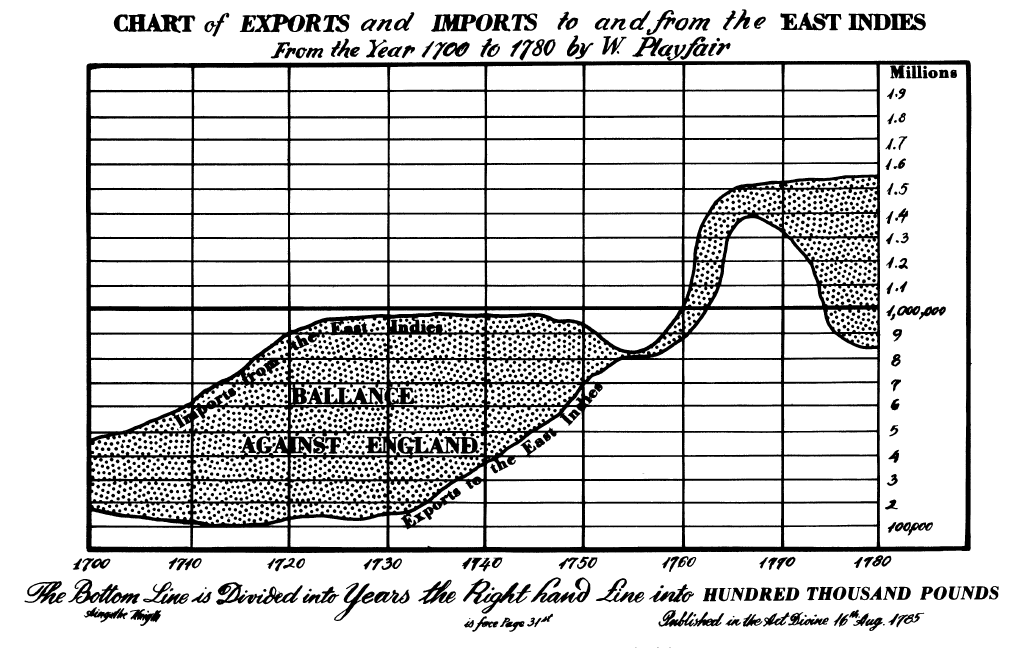
\includegraphics[width=.9\linewidth]{playfair_east_indies_gross}
\caption{\label{playfair}
Playfair's chart from the Commercial and Political Atlas (1786) showing the balance of trade between England and the East Indies.  In which years was the difference between imports and exports the highest? }
\end{figure}

\section{Illusions and Displays}
\subsection{Line width illusion}
An example of the  {\it line-width illusion} is displayed in  figure  \ref{playfair}. 


This chart displays the balance of trade between England and the East Indies as shown by William Playfair in his Commercial and Political Atlas, 1786 \cite{playfair, playfair2}.  One purpose of this chart is to demonstrate the difference between imports and exports in a particular year and its pattern over that time frame. The difference in exports and imports is encoded as the vertical difference between the lines. When observers are asked to sketch out the difference between exports and imports  \citep{cleveland:1984}, they very often  miss the steep rise in the difference between the lines in the years between about 1755 and 1765. Figure \ref{playfair2} shows the  actual difference between imports and exports. 



\begin{figure}
\centering
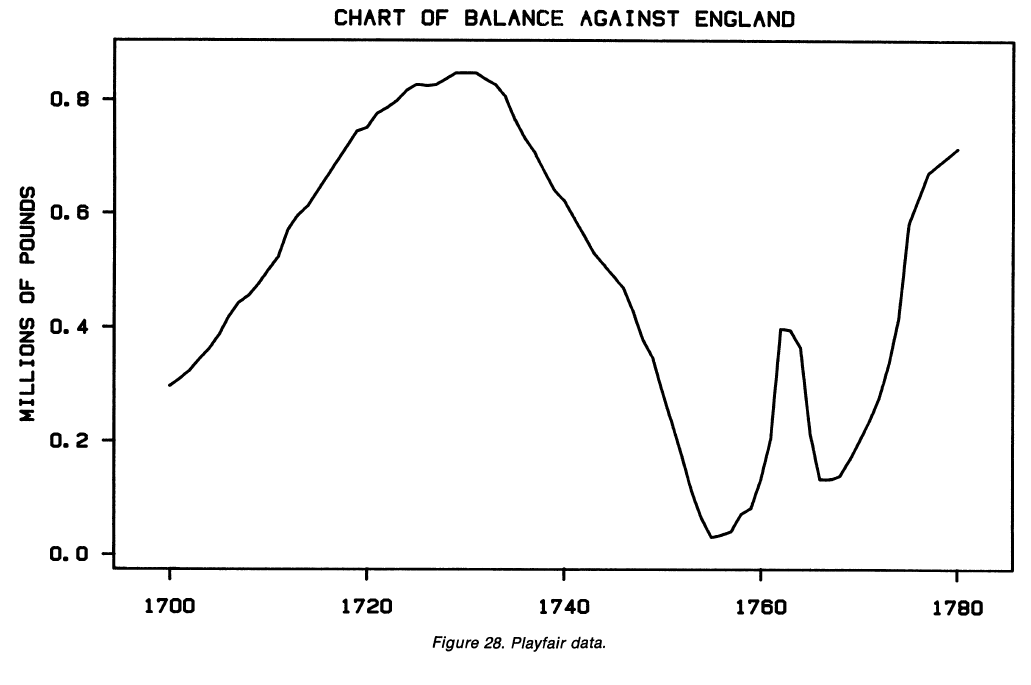
\includegraphics[width=.8\linewidth, height=.4\linewidth]{playfair_differenz_cleveland}
\caption{\label{playfair2}
Difference between exports and imports from England to and from the East Indies in the 18th century -- the steep rise in the difference around 1760  comes as a surprise to many viewers of the raw data in figure \ref{playfair}.  }
\end{figure}


This phenomenon  is known and widely discussed in statistical graphics literature \citep{cleveland:1984, tufte, wainer:2000, robbins:2005}. It  is due to our  tendency to assess distance between curves as the minimal (orthogonal) distance rather than the  vertical distance -- see sketch \ref{fig:linewidth} for a visual representation of both.


In the perception literature, this phenomenon is known as part of a group of geometrical optical misperceptions of a context-sensitive nature classified as M\"uller-Lyer illusions \citep{day:1991}. Interestingly, there seems to be a general agreement that this illusion exists, but a quantification of it is curiously absent from the literature. 

While we see the type of chart as shown in figure~\ref{playfair} proposed by Playfair quite commonly, particular in election years -- where these kind of charts are used to enable comparisons of support for several candidates, the recommendation from the literature is to avoid charts in which the audience is asked to do visual subtractions, and show these differences directly.

However, the line width illusion is not restricted to this situation only. We next discuss how other charts, such as the parallel sets plots \citep{kosara:2006}, are affected by it.
%We will first give an overview of  charts commonly used for displaying associations between categorical variables within the framework of parallel coordinate plots, and then discuss their performance with respect to the line width illusion. % based on user experiments.




%Figure \ref{sine-illusion} shows a screen shot of applet displaying the sine illusion. The sine illusion is closely related to the line width phenomenon -- the line segments in the are of the steepest slope of the sine curve appear to be the shortest: ``The illusion is explained in terms of a perceptual compromise between the vertical extent and the greater overall dimensions of the section at the turn of the sine-wave figure and is thereby held to be the same in principle as the M\"uller-Lyer illusion." \citep{day:1991}.
%M Bach's applet \citep{bach} gives the option to compensate the line length manually for its perceived shortcoming. The amount of compensation chosen turns out to be highly dependent on both the length of the vertical line segments and the amplitude of the sine function. The amplitude directly affects the slope -- the steeper  the slope the more compensation is necessary, see section \ref{distortion}  for a more detailed discussion and some results from a user study.
%
%
%\begin{figure}
%\centering 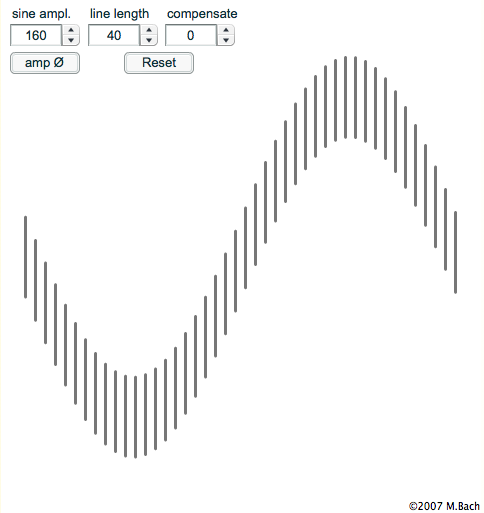
\includegraphics[width=.75\linewidth]{sine-illusion}
%\caption{Screenshot of an applet by M Bach \citep{bach} showing an example of a sine illusion. The applet is giving the possibility for compensating the line lengths in the regions with the highest slope. }
%\label{sine-illusion}
%\end{figure}




\subsection{Parallel set plots}


Parallel sets (parsets) have been introduced by R Kosara \citep{kosara:2006} as one way to visualize multivariate categorical data. Since their initial publication, they have spread to mass media outlets: see e.g. 
``How to understand risk in 13 clicks," BBC \citep{bbc:2009}.

  While retaining the %independent 
ability to visualize a large number of dimensions simultaneously that is the parallel coordinates' hallmark trade, Parallel Sets introduce the frequency scale that is a well-known feature of other categorical displays such as barcharts or mosaic plots \citep{hartigan:1981, friendly:1992, hofmann:2000, theus:1997}.
 Initially, frequencies of categories  were displayed as stacked boxes; in the later versions of Parallel Sets the boxes were reduced to simple lines \citep{parsetredesign}. Various implementations of parallel sets exist besides the original Java version, e.g.  J Davies introduced a d3 \citep{d3} version in  \citep{davies}.  The implementation of Parallel Sets-style displays in this paper is done in the software R \citep{R}. It retains the original box placeholders and does not enforce a tree hierarchy via color grouping. Section \ref{sec:implementation} gives details on the implementation, section \ref{sec:hierarchy} discusses dealings with hierarchical structures in the data.



\begin{figure}[hbtp]
\centering
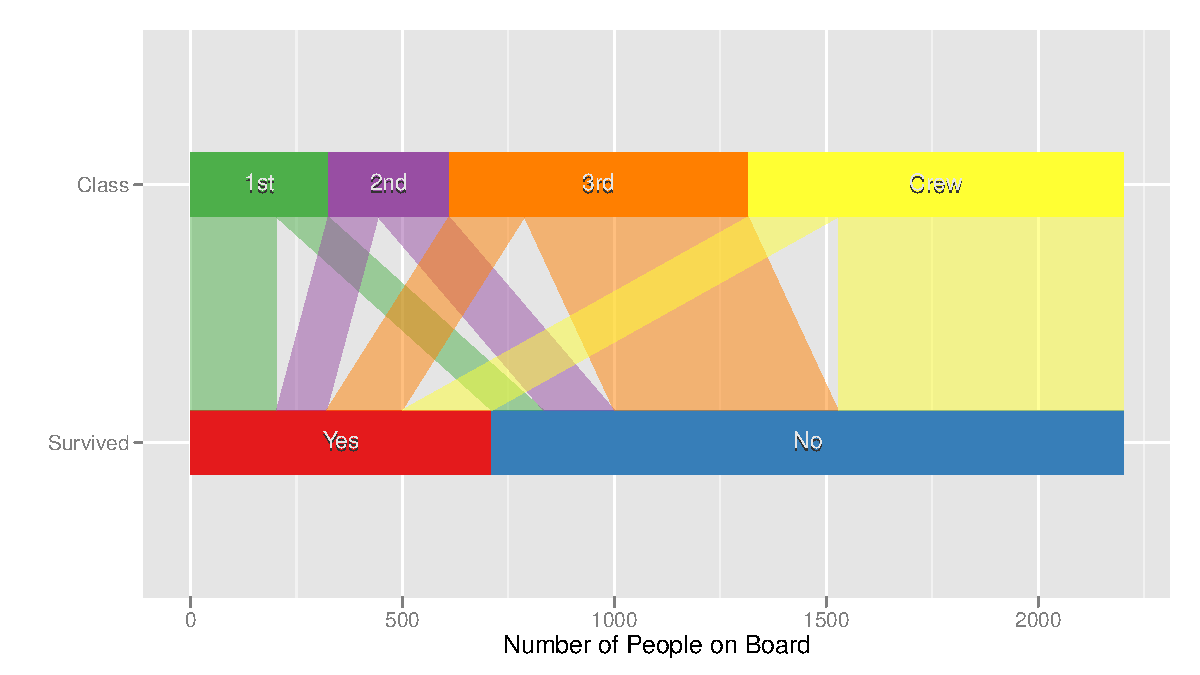
\includegraphics[width=.9\linewidth]{images/parset-titanic}
\caption{\label{question1a} Parallel sets plot showing the relationship between survival of the sinking of the HMS Titanic and class membership. }
\end{figure}
%XXX Description of parallel sets - and example


%%XXX PS and line-width illusion
%Parallel sets are  susceptible to the line width illusion: when we, for example, try to order passenger class and crew membership according to their respective numbers of survivors, we need to evaluate the width of the bands between upper and lower bars in figure \ref{question1a}.
%The  perceived width of the lines between the variables in figure \ref{question1a} would  lead us to assume that 1st class passengers had the highest number of survivors, followed by 3rd class passengers and about even numbers of survivors in the 2nd class  and  the crew. However, the  actual numbers are:


Figure \ref{question1a} gives an example for a two dimensional parallel sets plot investigating the relationship between class status and survival on board the HMS Titanic  \citep{dawson:1995}. Class status is recorded as either crew member or passengers, passengers are further classified as member of the first, second, or third class. 

 The top bar in figure \ref{question1a} shows the  variable Class. The bottom bar shows survival  as yes and no. Between the bars lines are drawn to visualize the relationship between class membership and  survival. 
  Based on the number of survivor and non survivors
  these bands are drawn from each class, and their (horizontal) width is proportional to the number of people they represent. 
% Based on the proportion of survivor and non survivors these bands are drawn from each class, and their (horizontal) width is proportional to the number of people they represent. 
%XXX PS and line-width illusion

This definition implies that lines are drawn under different angles, which makes the plots susceptible to the line width illusion. As an example, try to order the levels of variable 'class'  according to the number of survivors they have. In order to do that, we need to evaluate the width of the bands between upper and lower bars in figure \ref{question1a}.
The  perceived width of the lines between the variables in figure \ref{question1a} might  (and, as the responses from the survey in section \ref{results} show, does) lead us to assume that 1st class passengers had the highest number of survivors, followed by 3rd class passengers and about even numbers of survivors in the 2nd class  and  the crew. However, the  actual numbers are:
%
\begin{center}
\begin{tabular}{rrrrr}
& Crew & 1st & 2nd & 3rd \\ \hline
Survivors & 212 & 203 & 118 & 178\\
Non-Survivors & 673 & 122 & 167 &  528  
\end{tabular}
\end{center}
This identifies an order of crew, first class, third class, followed by second class as correct. 
We will discuss next how this finding relates to the line width illusion and how this helps us in quantifying the strength of the illusion.


%The plot in figure \ref{question1a} was created using an implementation of parallel sets written for the {\tt R} environment, found in the package {\tt ggparallel} (see section Implementation). A major distinction from the most recent {\tt ParSets v2.1} Java application is the choice to remain faithful to the structure of parallel sets proposed by Kosara in \citep{kosara:2006} and display frequency of each category as scaled boxes. Maintaining visual emphasis on the marginal probabilities of categories within a single dimension \citep{parsetredesign} reduces the impact of the line-width illusion for cognizant users.


%
\subsection{Strength of  line width illusion}\label{distortion}

%The difference between perceived and actual line width 
When visually evaluating lines of thickness greater than one, the line width illusion applies, only now the {\it edges} of a single line  take on the role of the separate curves. %in the parallel sets 
As above, there is a strong preference of evaluating the width of lines orthogonal to their slopes as opposed to horizontally (see figure \ref{fig:linewidth}), which is needed for a correct  evaluation of parallel sets-style displays.

Orthogonal $w_o$ and horizontal $w_h$ line widths are related -- the orthogonal line width depends on the angle (or slope) of the line:
\begin{equation}\label{adjust}
w_o = w_h \sin \theta,
\end{equation}
where $\theta$ is the angle of the line with respect to the horizontal line.

\begin{figure}[htbp]
\begin{center}
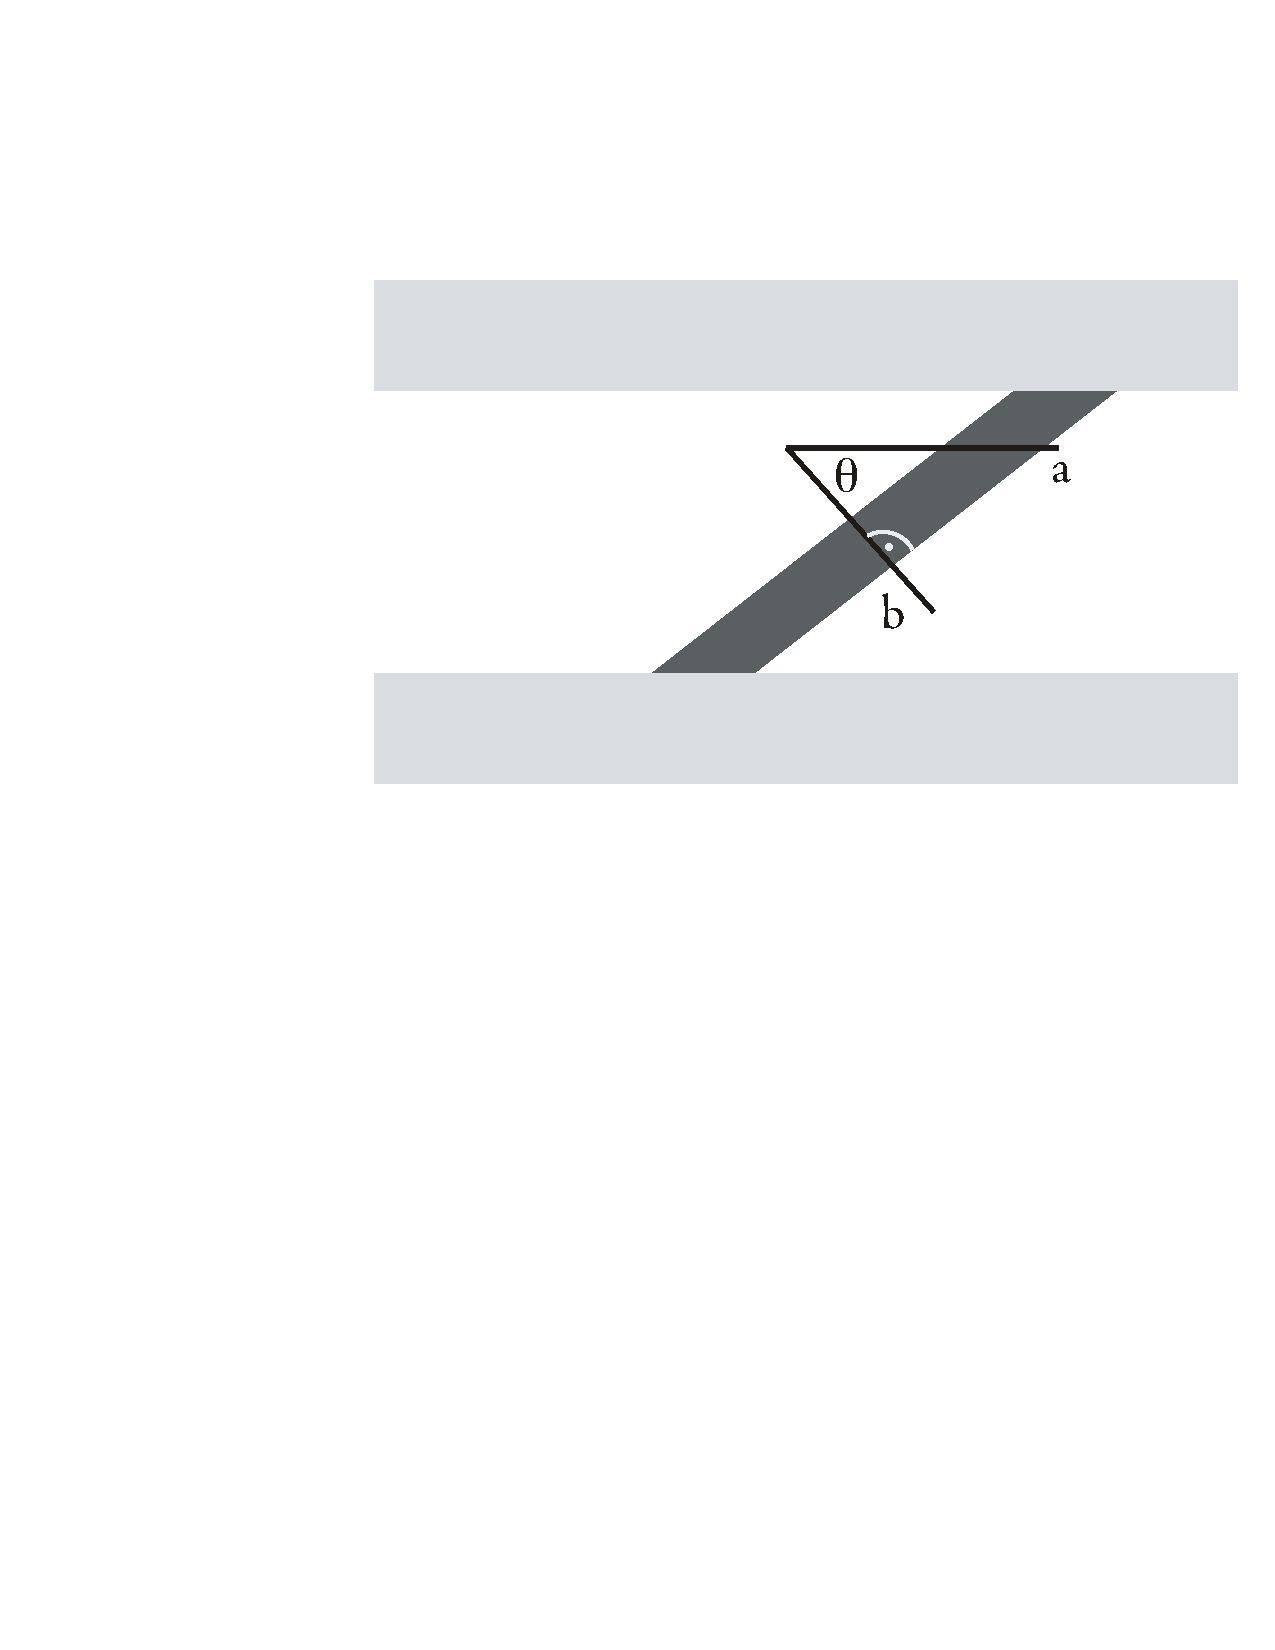
\includegraphics[width=0.6\linewidth]{images/linewidth}
\end{center}
\caption{\label{fig:linewidth}Sketch of line width assessments: (a) is showing  horizontal width, (b) shows  width orthogonal to the slope. From the survey results in section \ref{results} we can see that  observers associate line width more with  orthogonal width (b) than horizontal width (a).}
\end{figure}



%XXX aspect ratio


\begin{figure*}[htbp]
\begin{center}
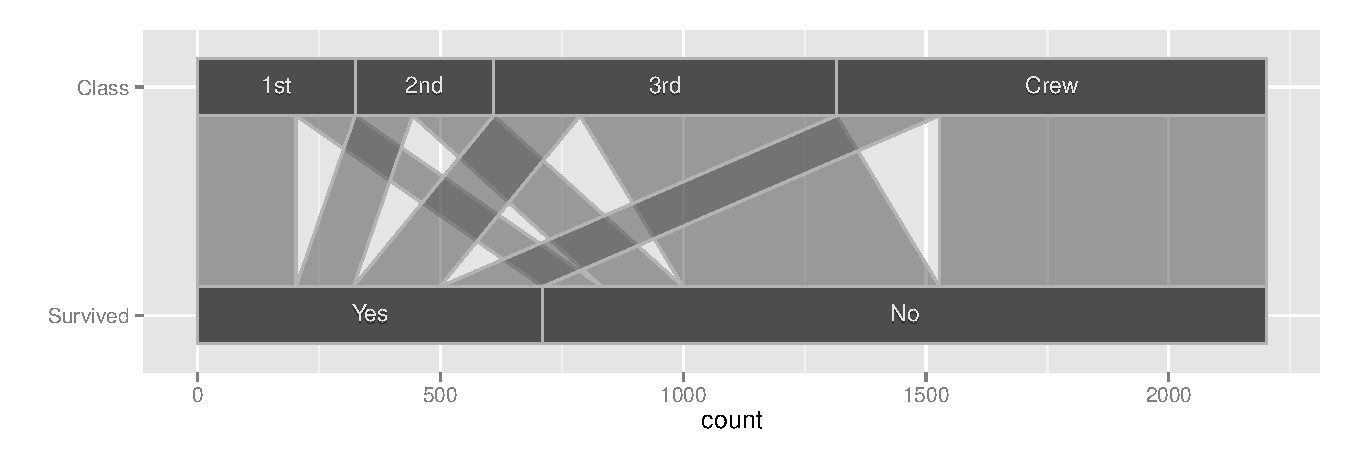
\includegraphics[height=1.5in]{images/aspect31-titanic.pdf}
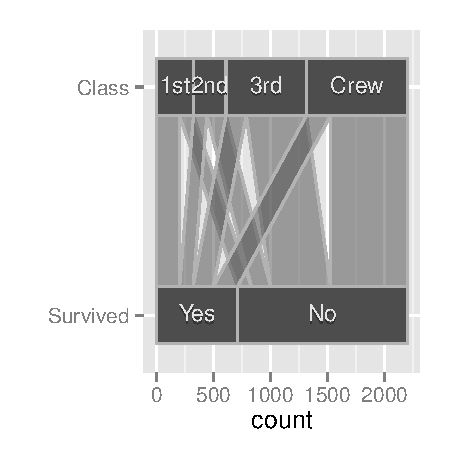
\includegraphics[height=1.5in]{images/aspect33-titanic.pdf}
\end{center}
\caption{\label{fig:aspect}Parallel sets plots of survival on the Titanic by class. Different aspect ratios  seemingly change the (orthogonal) line width, compare e.g. number of survivors in 3rd class and in the crew. }
\end{figure*}



The perceived slope of a line very much depends on the aspect ratio of the corresponding plot -- changing the height to width ratio of a display  will change our perception of the corresponding line widths, if they are not adjusted for the slope \cite{cleveland:1984}. This finding is not new, but its strength on our perception is surprising, as can be seen in the example of  figure \ref{fig:aspect}.  Again, survival and class membership on the Titanic is shown; the same parallel sets plot is shown twice in this figure, but with very different aspect ratios: in the  plot on the left the number of surviving 3rd class passengers seems to be about twice as big as the number of survivors among crew members, whereas in the plot on the right the lines have about equal (orthogonal) width. Obviously, this is not due to a change in numbers, nor a change in the way the plot is rendered. 

For parallel sets-style displays, the audience has an alternate visual cue when evaluating frequencies. Because height (width, when display is rotated 90 degrees) of a particular line is fixed for all line segments in the display, the width of a particular line segment is proportional to that segment's area. Comparison of area may be employed as a proxy or to augment line-width evaluations. This method of comparison is particularly troubling because it is prone to error in two scenarios commonly seen in Parallel Sets: (1) extreme aspect ratios of the rectangular shape occupied by thick line segments and (2) when comparing rectangles rotated relative to each other \citep{heer:2010, kong:2010}. Additionally, the incorrect perception and comparison of area provides contextual evidence that reinforce and strengthen distortion introduced by the line-width illusion.


Designers of good graphics have to accommodate changes in intuitive evaluation of the situation. While reordering categories and controlling the aspect ratio aids in reduction of audience potentially drawing wrong conclusions from a plot, none of these measures is enough to avoid all perceptual pitfalls due to the line width illusion.




%
%\begin{figure}[hbtp]
%\begin{center}
%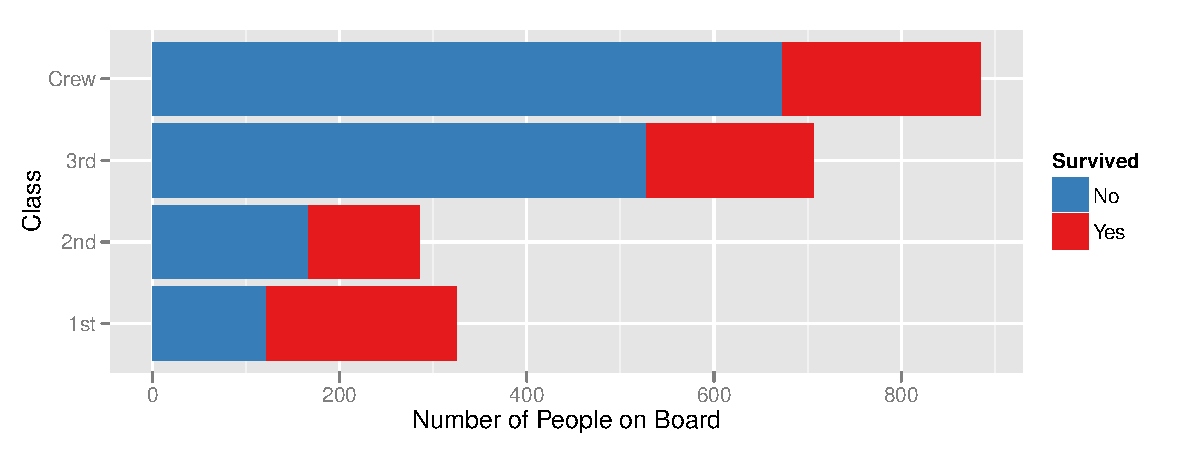
\includegraphics[width=.8\linewidth]{images/bar1-titanic}
%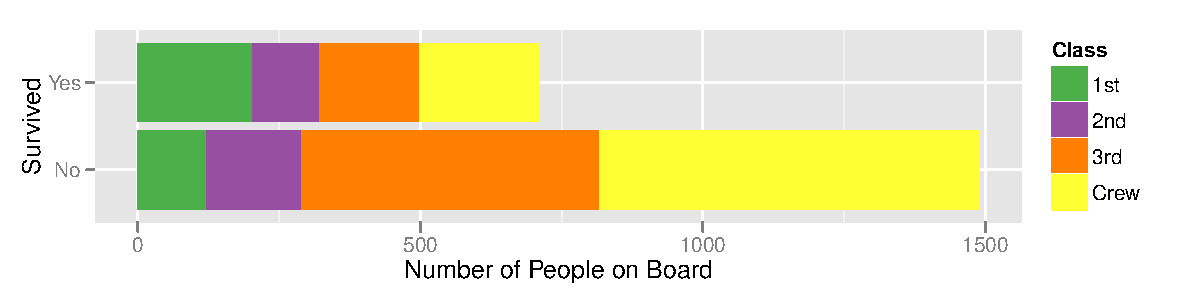
\includegraphics[width=.8\linewidth]{images/bar2-titanic}
%\end{center}
%\caption{\label{question1b} Barcharts showing Survival by Class for the Titanic Data.}
%\end{figure}



%In a preliminary survey participants were asked to order class  levels according to the number of survivors (from highest to lowest) based on  either the parallel sets plot of figure \ref{question1a} or the set of two barcharts in figure \ref{question1b} showing the same data.  
%
%% latex table generated in R 2.15.0 by xtable 1.7-0 package
%% Sat May 12 20:04:08 2012
%\begin{table}[ht]
%\begin{center}
%\begin{tabular}{rrrl}
%  \hline
% & barcharts & parallel sets & Correct \\ 
%  \hline
% 1st, 3rd, Crew,  2nd & 0 & 8 &  \\ 
%  1st, 2nd, Crew, 3rd & 0 & 4 &  \\ 
% 1st, Crew, 3rd, 2nd & 3 & 1 &  \\ 
%  Crew, 1st, 3rd, 2nd & 7 & 0 & * \\ 
%  Crew, 2nd, 3rd, 1st & 1 & 0 &  \\ 
%  Crew, 3rd, 2nd, 1st & 1 & 0 &  \\ 
%   \hline
%(all) & 12 & 13 &  \\ 
%   \hline
%\end{tabular}
%\caption{Overview of survey results: 7 out of 12 participants facing the barchart picked the correct order of `Crew, 1st, 3rd, 2nd' (highest number of survivors to lowest). None of the 13 participants evaluating the parallel set plot picked the correct result. }
%\label{tab:results}
%\end{center}
%\end{table}
%
%
%%  , , qid = 2
%%
%%                                              plottype
%%response                                       bar circos hammock
%%  1243                                           1      0       0
%%  2134                                           0      0       1
%%  3124                                           1      0       1
%%  4123                                          10      0      11
%%
%%, , qid = 3
%%
%%                                              plottype
%%response                                       bar circos hammock
%%  1342                                           1      0       1
%%  1432                                          10      0      11
%


% needed in second column of first page if using \IEEEpubid
%\IEEEpubidadjcol
\subsection{Hammock Plots}
%XXX Description of hammock plots and example

Hammock plots, introduced by M Schonlau in \citep{schonlau:2003}, provide an alternative to parallel sets that is adjusted for the line width illusion. This is done by  adjusting the --horizontal-- line width by  a factor of $\sin \theta$, as discussed in equation (\ref{adjust}). This adjustment makes the perceived --orthogonal-- line width to be proportional to the number of observations it represents. 
 Figure \ref{hammock} shows an example of a four dimensional hammock plot of the Titanic data. From top to bottom Class, Gender, Survival, and again Class are shown. 
\begin{figure}
%cols <- c(brewer.pal(name="Blues", 6)[-c(1,2)], rev(brewer.pal(name="Oranges", 3)[-1]), rev(brewer.pal(name="Greens",3)[-1]))
%ggparallel(names(titanic)[c(1,4,2,1)], order=c(0,1,1,0), method="hammock", ratio=.25, text.angle=0, titanic, weight="Freq") +
%  scale_fill_manual(values=cols, guide="none") +
%  scale_colour_manual(values=cols, guide="none") + coord_flip() 
%ggsave("hammock-titanic.pdf", width=6, height=8)
\centering
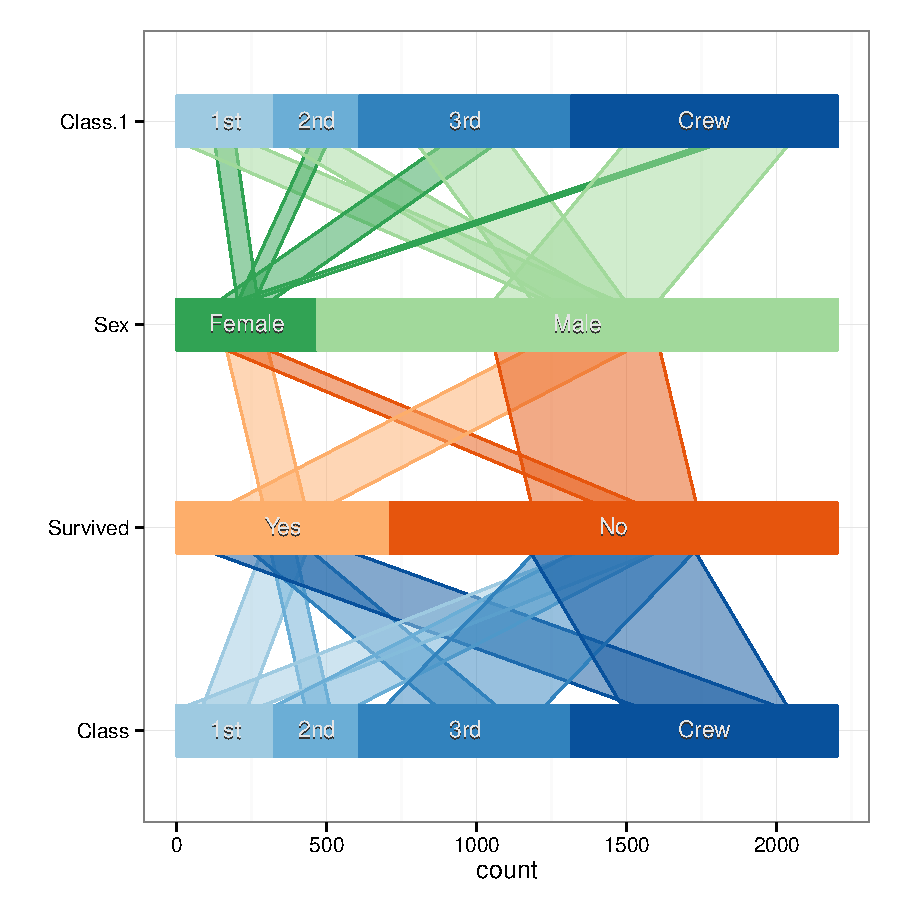
\includegraphics[width=\linewidth]{hammock-titanic}
\caption{\label{hammock} Hammock plot of the relationship between Class and Survival on the Titanic. }
\end{figure}

Similar to the parallel sets plot, the bars are divided according to class membership numbers.  Lines connect categories between neighboring bars, orthogonal line widths are representing the number of individuals in each combination. Unlike the parallel sets, the lines start from the middle of the bin and connect to the middle of the other variable's bins. 
%Line widths are adjusted in such a way, that the orthogonal width (see sketch \ref{fig:linewidth}) represents numbers.

Here, we see that barely any women were in the crew, while male crew members make up the second largest contingent overall. Overall a few more men survived than women, proportionally the situation is much different -- a much higher percentage of women survived than men. We also see, that more first class passengers survived than not, while second class passengers survival chances were about fifty-fifty. For third class passengers and crew members fewer members did  survive than not. 

As the adjustment of line widths is made with respect to the angle $\theta$, which itself depends on the aspect ratio of a plot, we need complete control over these properties of the plotting device when constructing Hammock plots  -- in our implementation (see below for details) we have dealt with this issue by fixing the aspect ratio. This is problematic in some situations, where the rendering has to be done without knowledge of the plotting device. 

Another problem that arises in evaluating hammock plots is that if an observer focuses on horizontal line width  the plots suffer from a {\it reverse line width illusion}:  judging the number of survivors by class in figure \ref{hammock} based on horizontal line width  results in an ordering of (largest to smallest) Crew, 3rd, 1st, and 2nd -- which is not correct either. Using horizontal width is inviting, since the lines are centered around the middle of a level, facilitating this  comparison. 

In this paper, we propose a new approach to visualizing relationships between categorical variables in a parallel coordinate plot setting, called the {\it common angle} display. 


\section{ Common Angle Plots}
\subsection{Construction}


\begin{figure}[htbp] %  figure placement: here, top, bottom, or page
%ggparallel(names(titanic)[c(1,4,2,1)], order=c(0,1,1,0), titanic, weight="Freq", text.angle=0) + 
%  scale_fill_manual(values=cols, guide="none") +
%  scale_colour_manual(values=cols, guide="none") + coord_flip() 
%ggsave("ca-titanic.pdf", width=6, height=6)
   \centering
   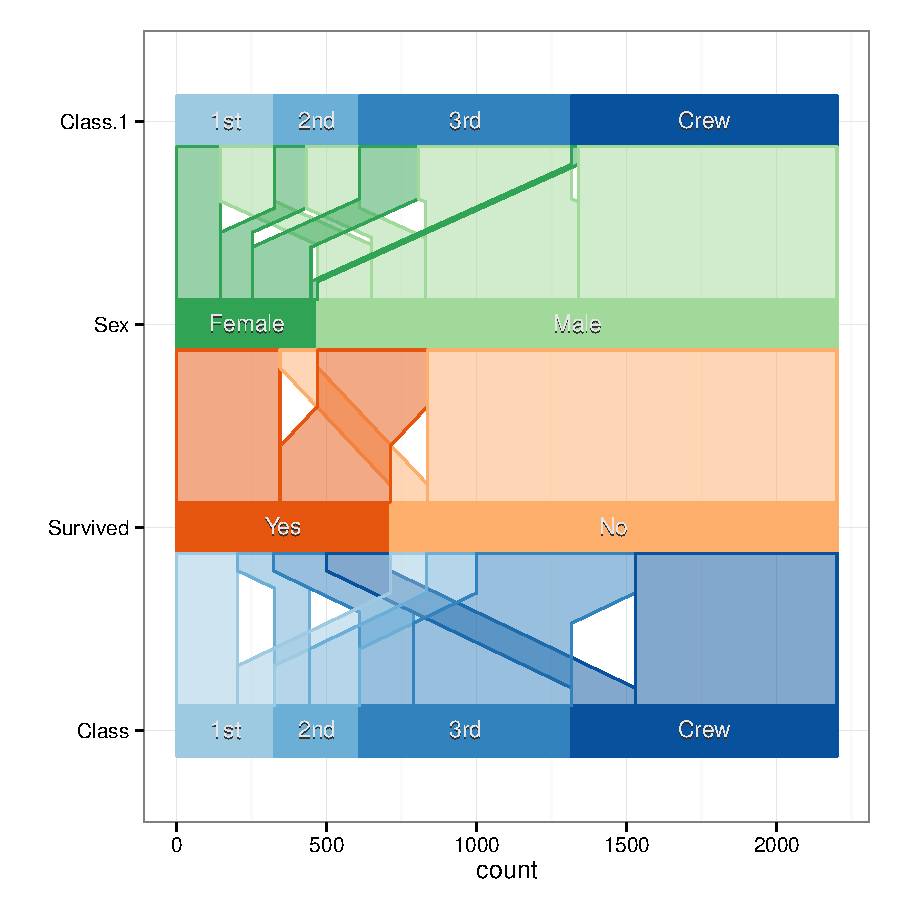
\includegraphics[width=\linewidth]{ca-titanic} 
   \caption{ \label{fig:ca-titanic} Common Angle plot of the Titanic data. }
  \end{figure}

Figure \ref{fig:ca-titanic} shows a common angle plot of the same data as the hammock plot.

As in the previously discussed display types ribbons are drawn between categories with widths  that are proportional to  the number of records they represent.

In order to ensure that  widths of all bands are  comparable without any distortion, their slopes  are artificially made the same in the following manner: 
assuming a vertical display as shown in figure \ref{fig:ca-titanic}, we modify  the connecting bands between  categories from a straight band  to a combination of a vertical  segment, a  segment under a pre-specified angle $\theta$, followed by another vertical  segment.  
The pre-specified angle $\theta$ (between the line and the vertical band) is given as --at most-- the angle of the longest connecting line between two categories of neighboring variables. 
This makes the width of ribbons  comparable without being affected by the distortion, as all ribbons are sharing at least one segment under the same angle. 

\subsection{Origins}
Historically, the common angle diagram has its roots in Sankey diagrams \citep{sankey:1898}. Sankey diagrams have their origin and main use of application in the area of industrial engineering. They are often used to show flows,  particularly, in the framework of energy consumption and losses within systems.
One of the most famous charts that can be classified as a Sankey diagram is Minard's map of Napoleon's march on Moscow \citep{minard:1812}. This map  shows the size of the army as a flow chart from West to East and the subsequent retreat. Usually, Sankey diagrams do not show a geographic co-variate, though. Modern uses of Sankey diagrams are discussed in  detail in \citep{schmidt:2008};  they can also be found in charts designed by Jen Christiansen, such as in \cite{jen3} and \cite{jen2}.

Shane Carter and Mike Bostock's chart `Over the Decades, How States Have Shifted' \citep{bostock:2012} is an example for a mixture of designs, involving a Sankey diagram.

%XXX http://www.jenchristiansen.com/ Jen Christiansen 
%http://jenchristiansen.com/?p=20
%Scientific American references 
%
%Sankey diagrams William O'Brien 'Preliminary Investigation of the use of Sankey diagrams ...'

\subsection{Extensions}
\subsubsection{Hammock-adjusted common angle plots}
As a logical next step in making ribbons comparable across all their parts and multiple variables, we can additionally adjust sloped parts of the ribbons using the hammock-adjustment described above. This leads to a representation as shown in figure \ref{adj.angle}. Note that ribbons no longer are required to fill the marginal bars. This choice was made to reduce the amount of overplotting resulting from the increase in width of the lines under an angle. The hammock adjustment results in re-introducing the aspect ratio of the display as a crucial quantity, and with that the implied dependency on  properties of the plotting device. 
\begin{figure}[hbtp]
%ggparallel(names(titanic)[c(1,4,2,1)], order=c(0,1,1,0), method='adj.angle', text.angle=0, weight="Freq", titanic, ratio=0.035) + 
%  scale_fill_manual(values=cols, guide="none") +
%  scale_colour_manual(values=cols, guide="none") + coord_flip() 
%ggsave("adj-angle.pdf", width=6, height=6)
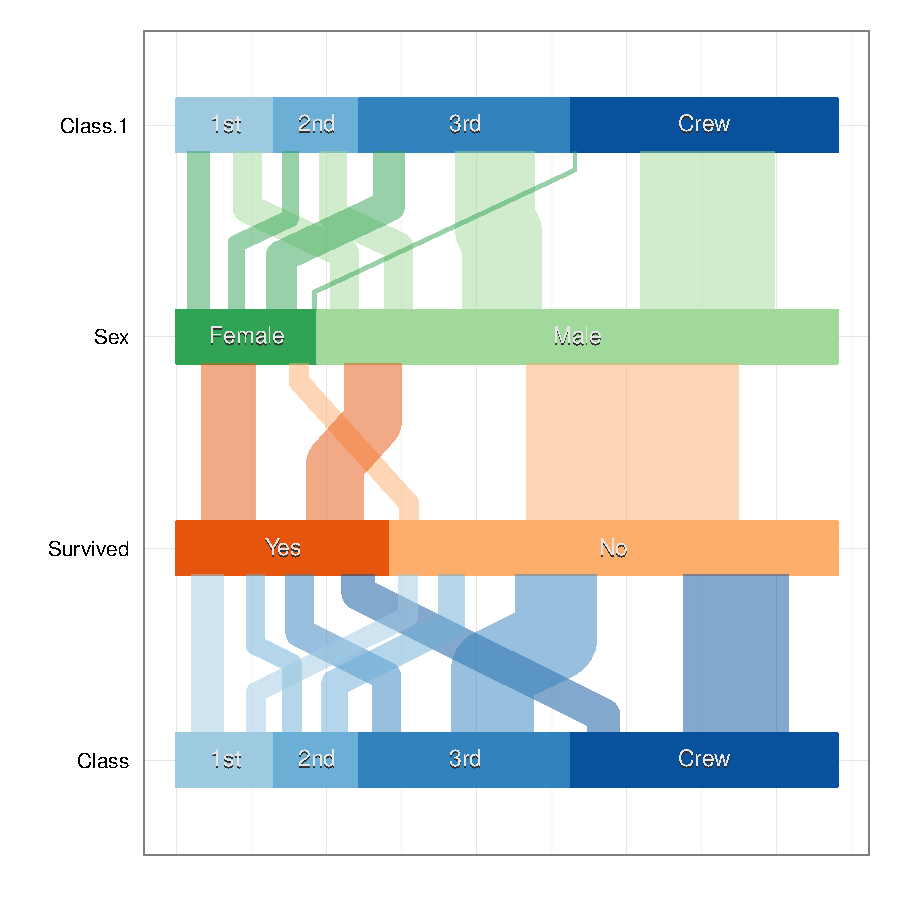
\includegraphics[width=\linewidth]{adj-angle}
\caption{\label{adj.angle} Adjusted common angle plot of the Titanic data.}
\end{figure}

\subsubsection{Hierarchies in Common Angle Displays}\label{sec:hierarchy}
In the original paper, parallel sets have been introduced to reflect a hierarchy of variables. In this paper, we have only used  sets of two-dimensional plots to focus on the association between pairs of variables. 
However, it is possible, to show hierarchies in all of the types of displays by defining the data correspondingly. 

Figure \ref{tit-hierarchy}
shows a common-angle plot  with a hierarchy: survivors of the disaster are marked in blue, non-survivors by orange. From top to bottom of the plot a hierarchy is drawn, considering first, survival, then gender, followed by age and finally, class membership. The coloring helps to keep track of survival status throughout the hierarchy, the common angle layout makes comparisons valid across all levels. This is of particular importance in hierarchical displays, as these displays, by definition, have a larger number of smaller groups than displays without a hierarchy acerbating problems induced by the line width illusion.

\begin{figure}[hbtp]
%titanic$SS <- with(titanic, interaction(Survived, Sex))
%titanic$SSA <- with(titanic, interaction(Survived, Sex, Age))
%titanic$CSSA <- with(titanic, interaction(Survived, Sex, Age, Class))
%
%
%tit <-titanic
%tit$Sex <- titanic$SS
%tit$Age <- titanic$SSA
%tit$Class <- titanic$CSSA
%
%cols <- rep(c("orange", "steelblue"),23)
%
%gg <- ggparallel(names(titanic)[c(1, 3, 2, 4)],  order=0, text.angle=0, label=FALSE, tit, weight="Freq", width=0.1) +
%  scale_fill_manual(values=cols, guide="none") +
%  scale_colour_manual(values=cols, guide="none") + coord_flip()
%
%#levels(titanic$Sex) <- c("Female", "Male")
%library(reshape)
%dfm <- melt(titanic, id.vars="Freq", measure.vars=c(1, 2, 3, 4))
%
%gg2 <- geom_bar(aes(x=variable, weight=Freq, group=value), width=.125, fill="grey40", colour="grey80", data=dfm)
%
%dfm$variable <- factor(dfm$variable, levels=levels(dfm$variable)[c(1,3,2,4)])
%
%label.stats <- ddply(dfm, .(variable, value), summarize,
%                     n = length(Freq),
%                     weight=sum(Freq)
%)
%maxWeight <- sum(label.stats$weight)/length(unique(label.stats$variable))
%label.stats$ypos <- cumsum(label.stats$weight)-(as.numeric(label.stats$variable)-1)*maxWeight
%label.stats$ypos <- label.stats$ypos-label.stats$weight/2
%
%text.offset <- 0
%label.stats$text.offset <- rep(text.offset, length=nrow(label.stats))
%
%varnames <- paste(unlist(vars), sep="|", collapse="|")
%label.stats$labels <- as.character(label.stats$value)
%gt1 <- geom_text(aes(x=as.numeric(variable), y=ypos-0.01, label=labels),
%                colour = "black", data=label.stats, angle=0, size=4)
%gt <- geom_text(aes(x=as.numeric(variable)+0.01+text.offset, y=ypos-0.01, label=labels),
%          colour = "grey90", data=label.stats, angle=0, size=4)
%
%gg + gg2 + gt1 + gt
%ggsave(file="ca-hierarchy.pdf", height=7, width=6)  
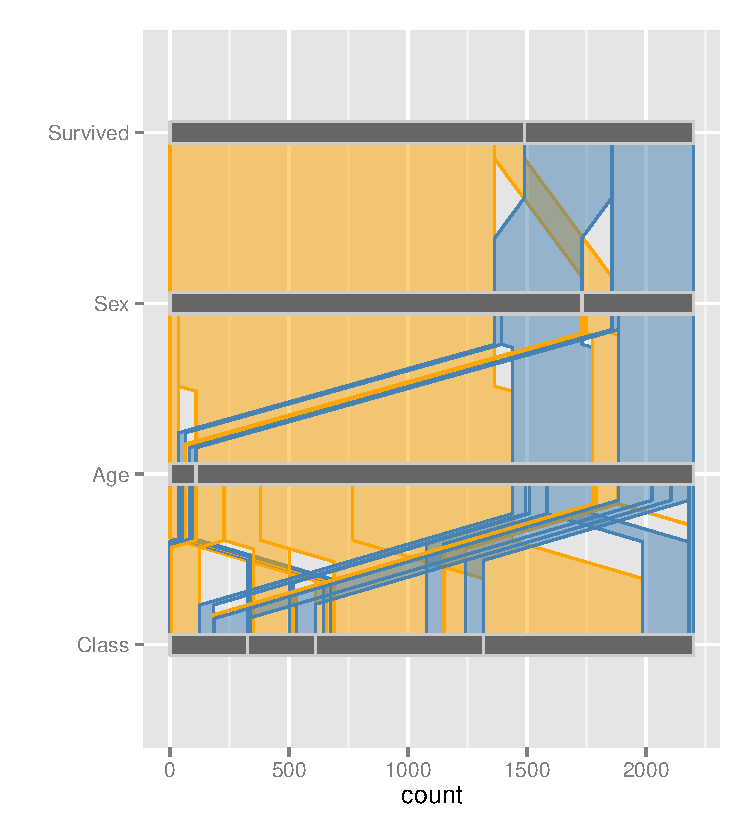
\includegraphics[width=\linewidth]{ca-hierarchy}
\caption{\label{tit-hierarchy} Common angle plot of the Titanic data using a hierarchical structure in the variable (cf. to parallel sets chart in \citep{davies}). }
\end{figure}


\section{Evaluation}
\subsection{Survey Design}
% description of general design
To determine the effectiveness of the common angle display, we conducted a user experiment in form of a survey asking participants to provide responses regarding the structure in two data sets with predominantly categorical variables.

 All individuals were presented with the same six questions, in two blocks of three questions each. The first block of questions investigated structures in the Titanic data set, including a follow-up of the survival-class ordering issue discussed earlier. Participants were exposed to one of the three types of displays discussed: a parallel sets plot, the Hammock plot of figure \ref{hammock}, or the common angle plot of  figure \ref{fig:ca-titanic}.
 
The second block  of questions regarded gene-pathway relationships in a dataset constructed from the UCSC Genome Browser \cite{ucsc:2002} for humane genome assembly. Ribbon widths here indicate the number of genes on a  chromosome that are active in a particular pathway. The pathways we focus on here, are involved in caffeine metabolism (hsa00232),  steroid biosynthesis (hsa00100), and hsa00982, which is involved with drug metabolism via the cytochrome P450 superfamily.  One important question when dealing with drug development are interactions with other drugs. Those interactions are more likely to happen when pathways use similar locations, e.g. gene CYP1A2 is involved in both  caffeine metabolism and the drug pathway -- clomipramine (an antidepressant) and caffeine both may act as a substrate. Chromosomes give a --very rough-- approximation to location. Connections between chromosomes and pathways are therefore interesting, when they show involvement of chromosomes in several pathways.
 
%See appendix for details regarding the survey demographics, and data.

%XXX discussion of datasets

%One application using 
Screening public databases of biochemical pathway and genetic sequence data to identify targets for further analysis is a common exploratory analysis task that benefits from visualization methods. One application may be to determine if a drug that is known to affect a particular pathway may also affect function on a different pathway. Such information would be useful in identifying new product markets or accurate warning labels. Another application would be discovery of colocalization between genes involved in multiple pathways; physical proximity is one indicator of evolutionary origin and may also provide clues regarding the mechanism that a pathway employs.
 
 Fits into Shneiderman's Visual Information Seeking mantra `Overview first, zoom and filter, then details-on-demand' \cite{shneiderman:96}
 
In Figure XXX the bottom bar shows three pathways: hsa00232, which is involved in caffeine metabolism; hsa00982, which is involved with drug metabolism via the cytochrome P450 superfamily; and hsa00100, which is involved in steroid biosynthesis. The top bar identifies chromosome location. A chromosome with ribbons connecting to multiple pathways are a physical target for drugs that possibly affect both paths. Gene CYP1A2 is involved in both caffeine metabolism and drug metabolism - clomipramine (an antidepressant) and caffeine both may act as a substrate for this gene. From a user perspective screening by the meta-location of chromosome reduces the colocalization question to one of searching for common elements from amongst 15 genes (number of genes active on a single chromosome for pathways hsa00232 and hsa00982) - reducing the search space by over 90\% (from 193 total genes listed for the pathways).

 
Participants were asked a second set of three questions (see appendix \ref{app2} for details) on this data set, but they were exposed to a  type of display different from the type accompanying questions from block 1.
  
This resulted in six different survey administrations, that were answered by similar number of participants: 

{ 

\scalebox{0.9}{
\begin{tabular}{rrrrrrr}
Block 1 & PS & CA & Ham & PS & CA & Ham \\ 
 Block 2 & CA & PS & PS & Ham & Ham & CA \\ \hline
\#responses &  9 &  8 &  9 &  7 & 11 & 8 \\ 
\end{tabular}}}

%% however the type of chart provided as reference for answering questions varied randomly among the types described previously. 
%%
%%In the survey, participants were first asked three questions regarding the titanic dataset, three questions regarding the gene dataset,  then two questions soliciting feedback regarding plot types, allowing for free response.

\noindent
This crossover design allows us to compare designs across different questions and data sets, while at the same time allowing to adjust for individuals' different skill sets. 
For the analysis, we first fit two linear mixed effects models, $M1$ and $M2$ -- the first one gives a general overview of comparing the designs, the second one further highlights the performance of the designs in each question.
We will then proceed to investigate some of the results in more detail.





\subsection{Results and Analysis}\label{results}
\subsubsection{Mixed effects models}
Answers for each question on the survey were assessed for correctness, giving us a binary variable of 1s and 0s, which we used to investigate performance of different designs. 

In a first model, $M1$, we are only interested in the overall difference in performance between designs. We can express this as a model of the form
\begin{equation}\label{model1}[M1]
\qquad\qquad y_i = \mu + d_{j(i)} + u_{k(i)} + \varepsilon_i \qquad\qquad
\end{equation}
where $y_i$ is the $i$th response, for $i = 1, ..., n$. $d_{j(i)}$ is the parameter measuring the effect of design $j$ ($j = C, H, P$ for \underline{C}ommon Angle, \underline{H}ammock plot, and \underline{P}arallel sets plot), $u_{k(i)}$ is the effect of participant's $k$ individual skills in evaluating these plots, $k \in \{1, ..., 52\}$. The assumption is that skills are independent and normally distributed with an expected value of zero and a variance of $\sigma_u^2$.
$\varepsilon_i$ is, similarly to a regular linear model, assumed to be independently distributed according to a normal distribution with mean of zero and variance $\sigma^2$.

Table \ref{coef1} gives an overview of the model coefficients and their estimates. The effect of the common angle design is used as a baseline, i.e all the effects shown are differences with respect to the performance of common angle plots. Both Hammock plots and Parallel sets plot have negative effects on the correctness of the response. This indicates a significantly worse performance of these designs than under the common angle design.

Table \ref{raw} shows percentages of correctness for each design and each question. Bold numbers indicate significantly different (worse) performance of a design compared to the common angle design. Note that question A.2 overall had the worst performance, parallel sets  exhibit significantly worse performance in four out of the six questions, Hammock plots are inferior to the common angle plot in two out the six questions. Note that in the last question Hammock plots have the best performance -- but this is does not  constitute a significant difference to the performance of the common angle design.
Also note, that the table shows raw percentages, i.e. these performance rates are not adjusted for skills of individuals. 

%xtable(summary(m1)@coefs)
% latex table generated in R 2.15.1 by xtable 1.7-0 package
% Fri Oct 12 09:08:11 2012
\begin{table}[ht]
\begin{center}
\begin{tabular}{lrrrrl}
  \hline
 & Estimate & Std. Error & z value & Pr($>$$|$z$|$) & \\ 
  \hline
$\mu$ & 1.72 & 0.24 & 7.04 & 0.00 & ***\\ [5pt]
  $d_C$& 0.00 & -- & -- & -- \\ 
  $d_H$ & -0.86 & 0.32 & -2.65 & 0.01 & ** \\ 
  $d_P$ & -1.31 & 0.32 & -4.07 & 0.00 & ***\\ 
   \hline
\multicolumn{5}{l}{Signif. codes:  0 `***' 0.001 `**' 0.01 `*' 0.05 `.' 0.1 ` ' 1 }
\end{tabular}
\end{center}
\caption{\label{coef1} Model fit for $M1$ measuring correctness of answers in the survey. The common angle design is used as baseline -- both Hammock plots and, to a larger degree, Parallel sets, show a significantly worse performance. }
\end{table}


%xtable(round(acast(survey, qu~design, fun=mean, value.var="correct")*100,3), digits=1)
% latex table generated in R 2.15.1 by xtable 1.7-0 package
% Fri Oct 12 11:21:19 2012
\begin{table}[ht]
\begin{center}
\begin{tabular}{rrrr}
  \hline
 & common & hammock & parallel \\ 
  \hline
 A1 & 86.0 & 76.5 & 81.2 \\ 
  A2 & 63.2 & {\bf 5.9} & {\bf 12.5} \\ 
  A3 & 73.7 & {\bf 17.6} & {\bf 25.0} \\ 
  B1 & 93.8 & 83.3 & 82.2 \\ 
  B2 & 68.8 & 68.8 & {\bf 6.7} \\ 
  B3 & 75.0 & 87.5 & {\bf 53.3} \\
   \hline
\end{tabular}
\end{center}
\caption{\label{raw} Raw percentages of correctness of responses for each question and design. Bold numbers indicate significant difference from common angle performances. }
\end{table}

Model $M2$ extends the first model by including both  effects for individual questions and the interaction effects with each design in the following form:
\begin{equation}\label{m2}[M2]
\quad y_i = \mu + d_{j(i)}  + q_{q(i)} + p_{j(i),q(i)} + u_{k(i)} + \varepsilon_i \quad
\end{equation}
Here, $q$ indicates the effects on performance for  each question, where $q(i)$ describes one of the questions $\{A1, A2, A3, B1, B2, B3\}$. $p$ is the parameter for the interaction effect of design and question, its index is a tuple consisting of a combination of a question and design. 

Figure \ref{fitted.m2} gives an overview of the goodness of fit of model $M2$ -- histograms of fitted values are drawn facetted by levels of the dependent variable. For correct responses fitted values are highly left skewed, with most values  above 0.5. For wrong answers we see a symmetric, if not quite as clear-cut picture: fitted values are skewed right. 
Overall, Model $M2$ is a significant improvement over model $M1$ (a corresponding log-likelihood ratio test is significant at a level of $<\!\!\!< 10^{-8}$).
Table \ref{model2} shows an overview of the  parameters and their estimates for model $M2$. After adjusting for individuals' skills Parallel sets perform significantly worse than common angle plots in three of the six questions. 

\begin{figure}
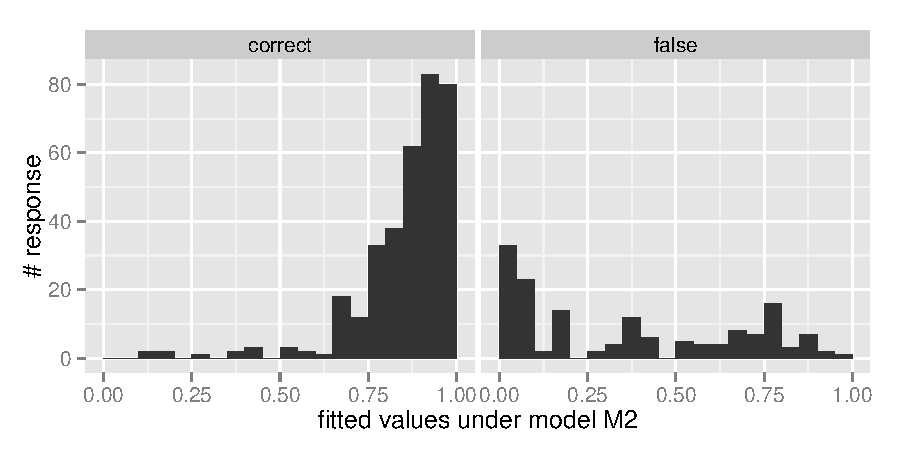
\includegraphics[width=\linewidth]{fitted-m2}
\caption{\label{fitted.m2} Histograms of fitted values under model $M2$, facetted by actual performance of participants. On the left, correct responses are shown. The histogram of fitted values is skewed to the right, with most values above 0.5. The histogram on the right corresponds to wrong answers. There are fewer wrong answers, and they tend to have low fitted values, but there are more false positives among them than false negatives for correct answers. }
\end{figure}

% xtable(summary(m4)@coefs)
% latex table generated in R 2.15.1 by xtable 1.7-0 package
% Fri Oct 12 09:12:32 2012
\begin{table}[ht]
\begin{center}
\begin{tabular}{rrrrrl}
  \hline
 & Estimate & Std. Error & z value & Pr($>$$|$z$|$) & \\ 
  \hline  
$\mu$ & 2.68 & 0.61 & 4.35 & 0.00  & ***\\ [5pt]
Design\\
  $d_C$ & 0.00 & -- & -- & -- \\ 
  $d_H$ & -1.06 & 0.83 & -1.28 & 0.20  \\ 
  $d_P$ & -0.57 & 0.86 & -0.66 & 0.51 \\ [5pt]
Questions\\
  $q_{A1}$ & 0.00 & -- & -- & -- \\ 
  $q_{A2}$  & -1.85 & 0.74 & -2.50 & 0.01 &* \\ 
  $q_{A3}$  & -1.11 & 0.77 & -1.44 & 0.15 \\ 
  $q_{B1}$ & 0.55 & 0.96 & 0.58 & 0.56 \\ 
  $q_{B2}$  & -1.69 & 0.88 & -1.91 & 0.06 &. \\ 
  $q_{B3}$  & -1.31 & 0.92 & -1.43 & 0.15 \\ [5pt]
 
Interaction \\
$p_{H, A1}$ &  0.00 & -- & -- & -- \\
$p_{P,A1}$ &  0.00 & -- & -- & -- \\
$p_{H, A2}$ &  -3.29 & 1.55 & -2.13 & 0.03 & *\\ 
$p_{P,A2}$ & -3.03 & 1.33 & -2.28 & 0.02 &*\\ 
$p_{H,A3}$ &-2.61 & 1.17 & -2.24 & 0.03  & * \\ 
$p_{P,A3}$ & -2.60 & 1.16 & -2.23 & 0.03 &*\\ 
$p_{H,B1}$ &-0.26 & 1.21 & -0.22 & 0.83 \\ 
$p_{P,B1}$ &-0.81 & 1.24 & -0.65 & 0.51 \\ 
$p_{H,B2}$ & 1.03 & 1.22 & 0.85 & 0.40 \\ 
$p_{P,B2}$  & -3.48 & 1.63 & -2.14 & 0.03 &*\\ 
$p_{H,B3}$ & 1.97 & 1.37 & 1.44 & 0.15 \\ 
$p_{P,B3}$ & -0.62 & 1.26 & -0.50 & 0.62 \\   
   \hline
\multicolumn{6}{l}{Signif. codes:  0 `***' 0.001 `**' 0.01 `*' 0.05 `.' 0.1 ` ' 1 }
\end{tabular}
\end{center}
\caption{\label{model2} Model fit for $M2$ measuring correctness of answers in the survey, detailing performance of designs on each question. All design comparisons are with respect to the common angle design. }
\end{table}


\begin{figure}
\centering 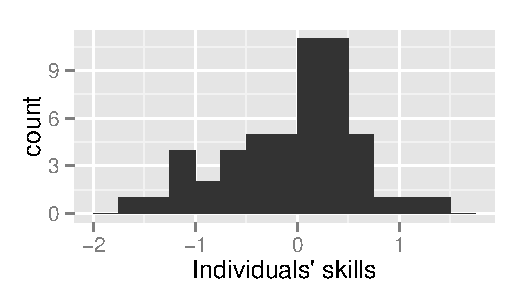
\includegraphics[width=.7\linewidth]{hist-skills}
\caption{\label{skills}Histogram of the predictions of subject-specific skills. }
\end{figure}	
Figure \ref{skills} shows an overview of the predicted skill for each participant under model $M2$. Skills are quite varied between  -1.52 and  1.34, but
a Kolmogorov-Smirnov test  does not show significant deviation from a normal assumption ($p$-value = 0.089).
On the scale of the dependent variable the range in individuals' skills translates to a $17.5 = e^{1.34 - (-1.52)}$ fold increase in the probability of answering a question on the survey correctly between participants with the best skill set and the worst.

In the next section we will investigate the results from the survey in further detail for some questions, and highlight the link to the line width illusion and its inverse.

\subsubsection{Evidence for line width illusions}

Question $A2$ asked participants to order  class levels  according to the number of survivors, fewest to highest. There are 4! = 24 distinct orderings of the levels, corresponding to all permutations of length 4. Some orderings are closer to one another than other orderings. The Cayley distance defines a way to quantify the distance between  each pair of permutations; the Cayley distance is defined as the minimal number of transpositions, i.e. swaps of two elements,  necessary to transform one permutation into the other.
We can make use of this distance to define a graph on the space of all permutations: let all permutations be nodes of the graph; for each two permutations with a Cayley distance of one, we add an edge to this graphs. This results in a regular graph of degree six, i.e. each  node is connected to six other nodes in the graph. The Cayley distance between any two nodes is then given as the length of the shortest path between the nodes through the graph.
Figure \ref{cubes} shows an overview of the permutation space together with an overview of the survey results. Each permutation is represent by one dot. 

The colored dots on top of the graph correspond to the responses from the survey - the size of the dots is proportional to the number of observers choosing this particular ordering. It becomes obvious from the three graphs in figure \ref{cubes} that
the answers to different designs occupy quite different regions, while answers based  on the same design are quite close --  usually separated by only one edge. 

The correct ordering, as well as the orderings assuming the line width illusion and its reverse are marked with symbols. Answers for the common angle design are centered around the correct answer, while responses to parallel sets are cluster around the response corresponding to the line width illusion. Due to the small number of responses to the hammock design a clear clustering of the answers is not recognizable, but the answer for the inverse line width illusion is among the responses. Table \ref{a2} gives an overview of all responses to question $A.2$. 

\begin{table}[ht]
\begin{center}
\begin{tabular}{rrrrl}
Order  & \rotatebox{90}{Common Angles}
& \rotatebox{90}{Hammock Plots}
& \rotatebox{90}{Parallel Sets} &\\
  \hline
  Crew, 1st, 3rd, 2nd &  &  2 &  \\ 
  2nd, 1st, 3rd, Crew &  &  6 &  & inverse illusion \\ 
   Crew, 3rd, 1st, 2nd &  &  1 &  1 \\ 
  2nd, 3rd, 1st, Crew & 2 & 7 & 1 \\ 
  2nd, 3rd, Crew, 1st & 12 &  1 &  2 & correct\\ 
  Crew, 3rd, 2nd, 1st &  2 &  &  \\ 
  3rd, 2nd, Crew, 1st &  1 &  &  \\ 
  1st, 2nd, 3rd, Crew &  1 &  &   \\ 
  1st, 3rd, Crew, 2nd &  1 &  &  2 \\ 
  Crew, 2nd, 3rd, 1st &  &  & 6 &  line width illusion\\  
  1st, 3rd, 2nd, Crew &  &  &  2 \\ 
  2nd, Crew, 3rd, 1st &  &  &  3 \\ 
   \hline
  Total & 19 & 17 & 16 \\ 
   \hline
\end{tabular}
\end{center}
\caption{\label{a2} Responses to question $A.2$: order levels of Class by the number of survivors (smallest to largest). }
\end{table}

%
Common angle displays show the best performance in terms of correctness (63.2\% on 19 responses), compared to a correctness of 11.8\% for parallel sets plots on 16 responses, indicating a significantly better performance of common angle plots at a level of 0.0027, based on a Mantel-Haenszel test (the difference in performance to Hammock plots is also significant at a level of 0.0006; but there is no significant difference in correctness between Hammock plots and parallel sets.).
While the intuitive assessment of line widths by their width orthogonal to slope is well known, it is surprising to see its strength: in this particular setting, it is strong enough to `shrink' the horizontally widest line for 6 out of 16 participants by at least  44\%, from 212 to below 118, and a further 3 participants perceived the shrinking to below 178, which constitutes a distortion of at least 16\%.

\begin{figure*}
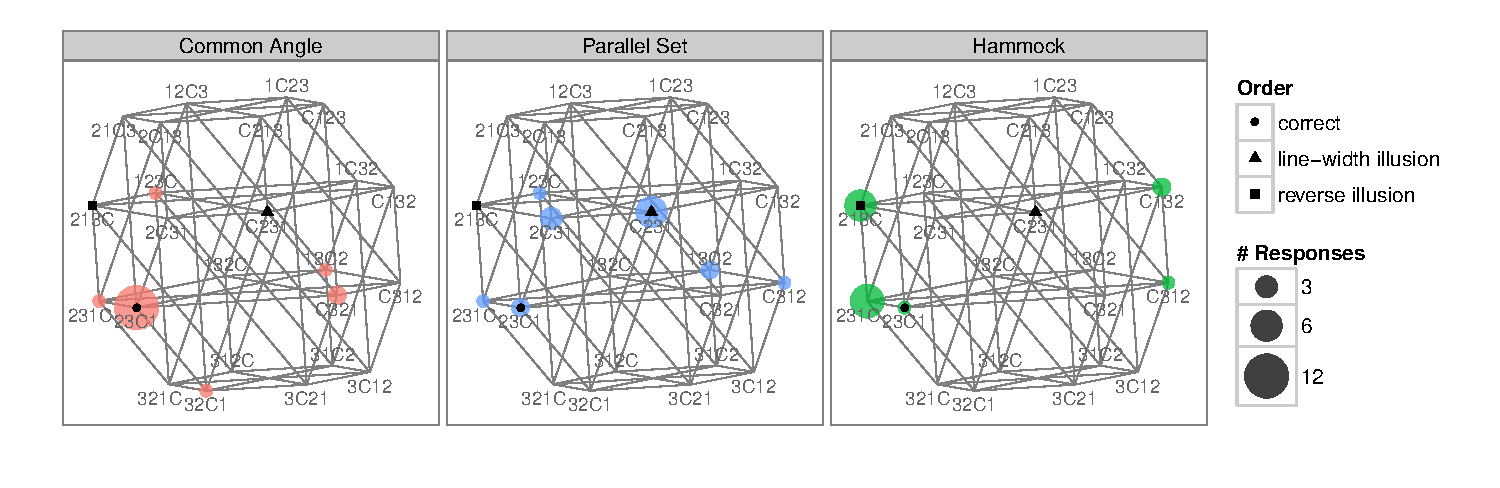
\includegraphics[width=\linewidth]{cubes}
\caption{Answers to question A.2 -- each node corresponds to a single ordering of the levels in variable 'Class'. Lines are drawn between orderings that are only one swap of levels apart. The colored dots show responses from the survey, their sizes depend on the number of responses for each ordering. }
\label{cubes}
\end{figure*}

Responses to question A.3 exhibit a similar pattern, see table \ref{a3}.

\begin{table}[ht]
\begin{center}
\begin{tabular}{rrrrl}
Order &  \rotatebox{90}{Common Angles}
& \rotatebox{90}{Hammock Plots}
& \rotatebox{90}{Parallel Sets} &\\
  \hline
c, b, a &  &  2 &  \\
a, b, c &  1 &  12 &  & inverse illusion\\ 
a, c, b & 14 &  3 &  4 & correct\\ 
b, c, a &  2 &  &  1 \\ 
c, a, b &  2 &  & 9 & line width illusion\\ 
b, a, c &  &  &  2 \\ 
 \hline
  Total & 19 &  17 & 16 \\ 
   \hline
\end{tabular}
\end{center}
\caption{\label{a3}Responses to question A.3: order combinations from smallest to largest, where 'a' is first class female, 'b' are male survivors, and 'c' are crew survivors. }
\end{table}
  
\begin{table}[ht]
\begin{center}
\begin{tabular}{clrrrl}
  Qu & Design & \rotatebox{90}{Correct} & \rotatebox{90}{Incorrect} & \rotatebox{90}{No Answer}   & Reason\\ \hline
  \hline
1 & common &   14 &  2 &   0 \\ 
   & hammock &   15 &  0 &   1 \\ 
 & parallel &   7 &   8 &   0 & line width illusion\\ \hline
2 & common &  16 &   0 &   0 \\ 
& hammock &   9 &   7 &   0 & inverse illusion\\ 
& parallel &  15 &   0 &   0 \\ \hline
3& common &  15 &   1 &   0 \\ 
& hammock &  16 &   0 &   0 \\ 
& parallel &  15 &   0 &   0 \\ 
   \hline
\end{tabular}
\end{center}
\caption{\label{tab:b1}Responses to question B.1 }
\end{table}


Table \ref{tab:b1} shows a summary to the  three questions of $B.1$ with possible answers ``agree", ``disagree", and ``don't know".
The first two questions are  examples, where the line width illusion, and its reverse will lead to answers that differ from the correct answer. Parallel sets plots are susceptible to the line width illusion, while hammock plots suffer from the reverse. The data shows that in about 50\% of the responses we can see this difference. 8 out of 15 answers for the parallel sets plots in question 1 deviate from the correct answer, and 7 out of 16 responses corresponding to hammock plots in question 2 show the wrong answer.


\subsection*{Opinion on CAs}
XXX which chart did you like better?

XXX breakdown of qualitative feedback

Out of the 14 cases where respondents saw both parallel sets and common angle plots....

8* (57\%) cited comparison of width, area or "size"
3* (21\%) cited the angle of incidence
2 (14\%) cited the underlying data structure  - fewer variables, "logical"
1 (7\%) said choice was "easier"
1 (7\%) gave other responses - asked for clarification of the plot type,


*one person cited both area and angle of incidence

12 people preferred common angles


\section{Implementation}\label{sec:implementation}

All  of the discussed variants of parallel coordinate plots for categorical data are implemented as part of the package {\tt ggparallel} based on the {\tt ggplot2} \cite{ggplot2} plotting framework in the software {\tt R} 2.15.1 \citep{R}. The  {\tt ggparallel} package is freely available from CRAN (\url{http://www.r-project.org/}).
The colors for the plots have been chosen using color schemes from the ColorBrewer project  \cite{colorbrewer} , as implemented in the R package {\tt RColorBrewer}  \cite{RColorBrewer} .


\section{Conclusion}
%
% What did we do? 
We have been investigating different types of plots used for visualizing structures between categorical variables, the parallel sets display, and the hammock display.
We have presented strong evidence that Hammock plots and parallel sets suffer from a type of M\"uller Lyer illusion, which we have coined the line width illusion and its reverse. 
We have introduced common angle plots as a measure to avoid the line width illusions and found strong evidence that  the performance of the common angle plot is not affected by these line width illusions and significantly better in these situations.

We have presented overwhelming evidence in the `case against straight lines', in particular when line width is encoding quantitative information. Even though straight lines are the simple and mathematically perfect solution to represent  connections  between levels of two variables, they are far from optimal for the peruser of the chart in two ways: firstly by the line width illusion in Parallel sets plots, and secondly by the reverse of the line width illusion after the adjustment in Hammock Plots.   Parallel Sets are affected by the line width illusion, which is a clash between need and nature -- mathematics tells us that we  need to assess line widths in a vertical or horizontal fashion to get a correct evaluation of the encoded information. This clashes with a strong innate tendency to evaluate  widths of lines orthogonally to their  direction. 
Hammock plots are adjusting for the line width illusion by changing the  width corresponding to the slope of the line segment. However, this makes either end of the segments susceptible to the reverse line width illusion. We found strong support in the survey we conducted for the existence of both the line width illusion in common angle plots and the reverse in Hammock plot. By giving up on the paradigm of straight lines for drawing connections between levels in the common angle display, we are able to circumnavigate both illusions, and present an illusion-free alternative that encodes the same information as the widely used Parallel sets plots or the Hammock plots.



%
\appendix
%\subsection*{Demographics of the pre-cursory survey I}\label{app1}
%33 students, staff and faculty from Iowa State University participated in the survey investigating the strength of the perceptual line width distortion. The Qualtrics system \cite{} was used to create the survey and all students, staff and faculty from programs in Statistics, Bioinformatics and Computational Biology and Human Computer Interaction were invited to participate by email. No personally identifiable information was collected, nor was any compensation offered. Participants used their own personal computing devices to access the survey. A majority of participants used WoW64 (Windows 32-bit or Windows 64-bit), with the next most common operating system Intel Mac OS X10.6.8 (Snow Leopard). The preferred choice of browser was  Chrome, followed by Firefox. For two participants, the Qualtrics survey software was unable to capture operating system or browser information.
%
%One question in this survey asked participants to rank the number of survivors in the titanic dataset by class. The results are summarized in table  \ref{tab:results} .


%No participants chose to do so using internet explorer. 

% ## operating system
% summary(df2$Q2_3_TEXT)
% #                      Intel Mac OS X 10_6_8 Intel Mac OS X 10_7_3   Intel Mac OS X 10.6          Linux x86_64 
% #                    2                     7                     4                     1                     3 
% #               rv:6.0                Ubuntu                 WOW64 
% #                    1                     1                    14 
% 
% ## browser info
% ### NOTE: I discovered after the survey went out that IE renders the html code for the training data poorly
% summary(df2$Q2_1_TEXT)
% #         Chrome Firefox  Safari 
% #      2      16      10       5 

% In contrast to that, a second question asking participants to order class levels according to survival {\it rates} of members did not yield any indication that parallel sets were performing less efficiently than barcharts; 11 out of 12 (barcharts) and 12 out of 13 (parallel sets) participants were able to answer this question correctly. The answer was also based on either figure \ref{question1a} or \ref{question1b}. While the line width illusion is present, its effect for this instance is not strong enough to have an impact on the order of the results.



\subsection*{Survey }\label{app2}
All students, staff and faculty from Iowa State University programs in Statistics, Bioinformatics and Computational Biology and Human Computer Interaction were invited to participate by email. 93 individuals accessed the survey, with 47 individuals submitting responses for all questions. Participants used their own personal computing devices to access the survey, which was created using the  Qualtrics Labs, Inc software (\url{www.qualtrics.com}). No personally identifiable information was collected, nor was any compensation offered. At the survey start, participants were presented a brief tutorial regarding the different plot types.  \\

\noindent The questions pertaining to the titanic dataset were: \\ \\
\begin{itemize}
\item[A.1]\emph{Agree, Disagree or Don't Know/Can't Determine with the following statements:}
\begin{itemize}
\item There were an approximately equal number of Male and Female Survivors
\item The group with largest number of travelers was Female Survivors
\item There were more Male Non-Survivors than number of males in First and Second Class Combined
\end{itemize}

\item[A.2]\emph{Order the categories of Class by number Survived, fewest to most.} 
\begin{itemize}
\item 1st
\item 2nd 
\item 3rd
\item Crew
\end{itemize}

\item[A.3]\emph{Order the following groups by number, fewest to most}
\begin{itemize}
\item 1st Class female passengers
\item Male Survivors
\item Crew Survivors
\end{itemize}
\end{itemize}


\noindent \\  The questions pertaining to the gene dataset were: 


\begin{itemize}
\item[B.1]\emph{Agree, Disagree or Don't Know/Can't Determine with the following statements:}
\begin{itemize}
\item There are about the same number of genes in the group "steroid biosynthesis:chromosome 1" as in the group "caffeine metabolism: chromosome 8"
\item The group with the greatest number of genes is "drug metabolism:chromosome 4"
\item there are more genes involved in the group "drug metabolism: chromosome 1" than all genes involved in the caffeine metabolism pathway
\end{itemize}

\item[B.2]\emph{Order the following chromosomes by number of genes involved in steroid biosynthesis pathway, fewest to most.}
\begin{itemize}
\item chromosome 1
\item chromosome 4
\item chromosome 8 
\item chromosome X
\end{itemize}

\item[B.3]\emph{Order the following chromosomes by number of genes involved, fewest to most.}
\begin{itemize}
\item steroid biosynthesis :: chromosome X
\item steroid biosynthesis :: chromosome 4
\item drug metabolism :: chromosome X
\end{itemize} 
\end{itemize} 

%\noindent \\Participants were randomly assigned to one of six blocks, each of approximately equal size. While individuals in all blocks were presented with the same questions and datasets in the order shown above, each block was presented with a unique ordering of only two of the plot types (e.g parallel sets and hammock plot; common angles and parallel sets, etc) to use as reference when respon. This study design structure was imposed, in part,  to encourage participation by reducing the amount of time for survey completion. Completion of all survey questions was anticipated to take 10 - 15 minutes.

\subsection*{Data and preprocessing}
Data for questions A1, A2 and A3 in survey 2 were previously published in: \citep{dawson:1995}.

Data for questions B1, B2 and B3 in survey 2 was obtained using the UCSC Genome Browser \cite{ucsc:2002} for humane genome assembly (hg18, May2006). The data was subsetted for genes involved in pathways hsaXXX (drug metabolism), hsaXXX (caffeine metabolism), and hsaXXX (steroid biosynthesis). From this data, genes active on selected chromosomes were displayed in plots.

All data manipulation was performed  using software {\tt R} 2.15.1 \citep{R} with Bioconductor package KEGG.db \cite{kegg}
%
\subsection*{Participants' demographics}
XXX Add breakdown of operating system

% use section* for acknowledgement
\ifCLASSOPTIONcompsoc
  % The Computer Society usually uses the plural form
  \section*{Acknowledgments}
\else
  % regular IEEE prefers the singular form
  \section*{Acknowledgment}
\fi


The survey for this study was carried out with approval from  IRB-ID 12-204.


% Can use something like this to put references on a page
% by themselves when using endfloat and the captionsoff option.
\ifCLASSOPTIONcaptionsoff
  \newpage
\fi



% trigger a \newpage just before the given reference
% number - used to balance the columns on the last page
% adjust value as needed - may need to be readjusted if
% the document is modified later
%\IEEEtriggeratref{8}
% The "triggered" command can be changed if desired:
%\IEEEtriggercmd{\enlargethispage{-5in}}

% references section

% can use a bibliography generated by BibTeX as a .bbl file
% BibTeX documentation can be easily obtained at:
% http://www.ctan.org/tex-archive/biblio/bibtex/contrib/doc/
% The IEEEtran BibTeX style support page is at:
% http://www.michaelshell.org/tex/ieeetran/bibtex/
\bibliographystyle{IEEEtran}
% argument is your BibTeX string definitions and bibliography database(s)
\bibliography{references}
%
% <OR> manually copy in the resultant .bbl file
% set second argument of \begin to the number of references
% (used to reserve space for the reference number labels box)
%\begin{thebibliography}{1}
%
%\bibitem{IEEEhowto:kopka}
%%This is an example of a book reference
%H. Kopka and P.W. Daly, \emph{A Guide to {\LaTeX}}, third ed. Harlow, U.K.: Addison-Wesley, 1999.
%
%
%%This is an example of a Transactions article reference
%%D.S. Coming and O.G. Staadt, "Velocity-Aligned Discrete Oriented Polytopes for Dynamic Collision Detection," IEEE Trans. Visualization and Computer Graphics, vol.?14,? no.?1,? pp. 1-12,? Jan/Feb? 2008, doi:10.1109/TVCG.2007.70405.
%
%%This is an example of a article from a conference proceeding
%%H. Goto, Y. Hasegawa, and M. Tanaka, "Efficient Scheduling Focusing on the Duality of MPL Representation," Proc. IEEE Symp. Computational Intelligence in Scheduling (SCIS '07), pp. 57-64, Apr. 2007, doi:10.1109/SCIS.2007.367670.
%
%%This is an example of a PrePrint reference
%%J.M.P. Martinez, R.B. Llavori, M.J.A. Cabo, and T.B. Pedersen, "Integrating Data Warehouses with Web Data: A Survey," IEEE Trans. Knowledge and Data Eng., preprint, 21 Dec. 2007, doi:10.1109/TKDE.2007.190746.
%
%%Again, see the IEEEtrans_HOWTO.pdf for several more bibliographical examples. Also, more style examples
%%can be seen at http://www.computer.org/author/style/transref.htm
%\end{thebibliography}

% biography section
% 
% If you have an EPS/PDF photo (graphicx package needed) extra braces are
% needed around the contents of the optional argument to biography to prevent
% the LaTeX parser from getting confused when it sees the complicated
% \includegraphics command within an optional argument. (You could create
% your own custom macro containing the \includegraphics command to make things
% simpler here.)
%\begin{biography}[{\includegraphics[width=1in,height=1.25in,clip,keepaspectratio]{mshell}}]{Michael Shell}
% or if you just want to reserve a space for a photo:

\begin{IEEEbiography}{Heike Hofmann}
Biography text here.
\end{IEEEbiography}

\begin{IEEEbiography}{Marie Vendettuoli}
Biography text here.
\end{IEEEbiography}

% if you will not have a photo at all:
%\begin{IEEEbiographynophoto}{John Doe}
%Biography text here.Biography text here.Biography text here.Biography text here.Biography text here.Biography text here.Biography text here.Biography text here.Biography text here.Biography text here.Biography text here.Biography text here.Biography text here.Biography text here.Biography text here.Biography text here.Biography text here.Biography text here.Biography text here.Biography text here.Biography text here.Biography text here.Biography text here.Biography text here.Biography text here.Biography text here.Biography text here.Biography text here.Biography text here.Biography text here.Biography text here.Biography text here.
%\end{IEEEbiographynophoto}
%
%% insert where needed to balance the two columns on the last page with
%% biographies
%%\newpage
%
%\begin{IEEEbiographynophoto}{Jane Doe}
%Biography text here.Biography text here.Biography text here.Biography text here.Biography text here.Biography text here.Biography text here.Biography text here.Biography text here.Biography text here.Biography text here.Biography text here.Biography text here.Biography text here.Biography text here.Biography text here.Biography text here.Biography text here.Biography text here.Biography text here.Biography text here.Biography text here.Biography text here.Biography text here.Biography text here.Biography text here.Biography text here.Biography text here.
%\end{IEEEbiographynophoto}

% You can push biographies down or up by placing
% a \vfill before or after them. The appropriate
% use of \vfill depends on what kind of text is
% on the last page and whether or not the columns
% are being equalized.

%\vfill

% Can be used to pull up biographies so that the bottom of the last one
% is flush with the other column.
%\enlargethispage{-5in}



% that's all folks